\begin{frame}{McGill NeuroTech: student-built TMS research hardware}
  \begin{columns}[c,onlytextwidth]
    \column{.57\textwidth}
      \small
      \NTXPoint{A new hardware-team preprint}{Lapatrie and collaborators: a low-cost monophasic transcranial magnetic stimulator.}
      \NTXPoint{About US\$700 in parts}{Off-the-shelf components and a custom coil; bench equipment is additional.}
      \NTXPoint{Build, characterize, share}{Measured magnetic fields inform cortical-field models. A concrete example of ambitious student research.}
      {\scriptsize Research prototype --- not approved for human stimulation or clinical use.\par}
    \column{.39\textwidth}
      \centering
      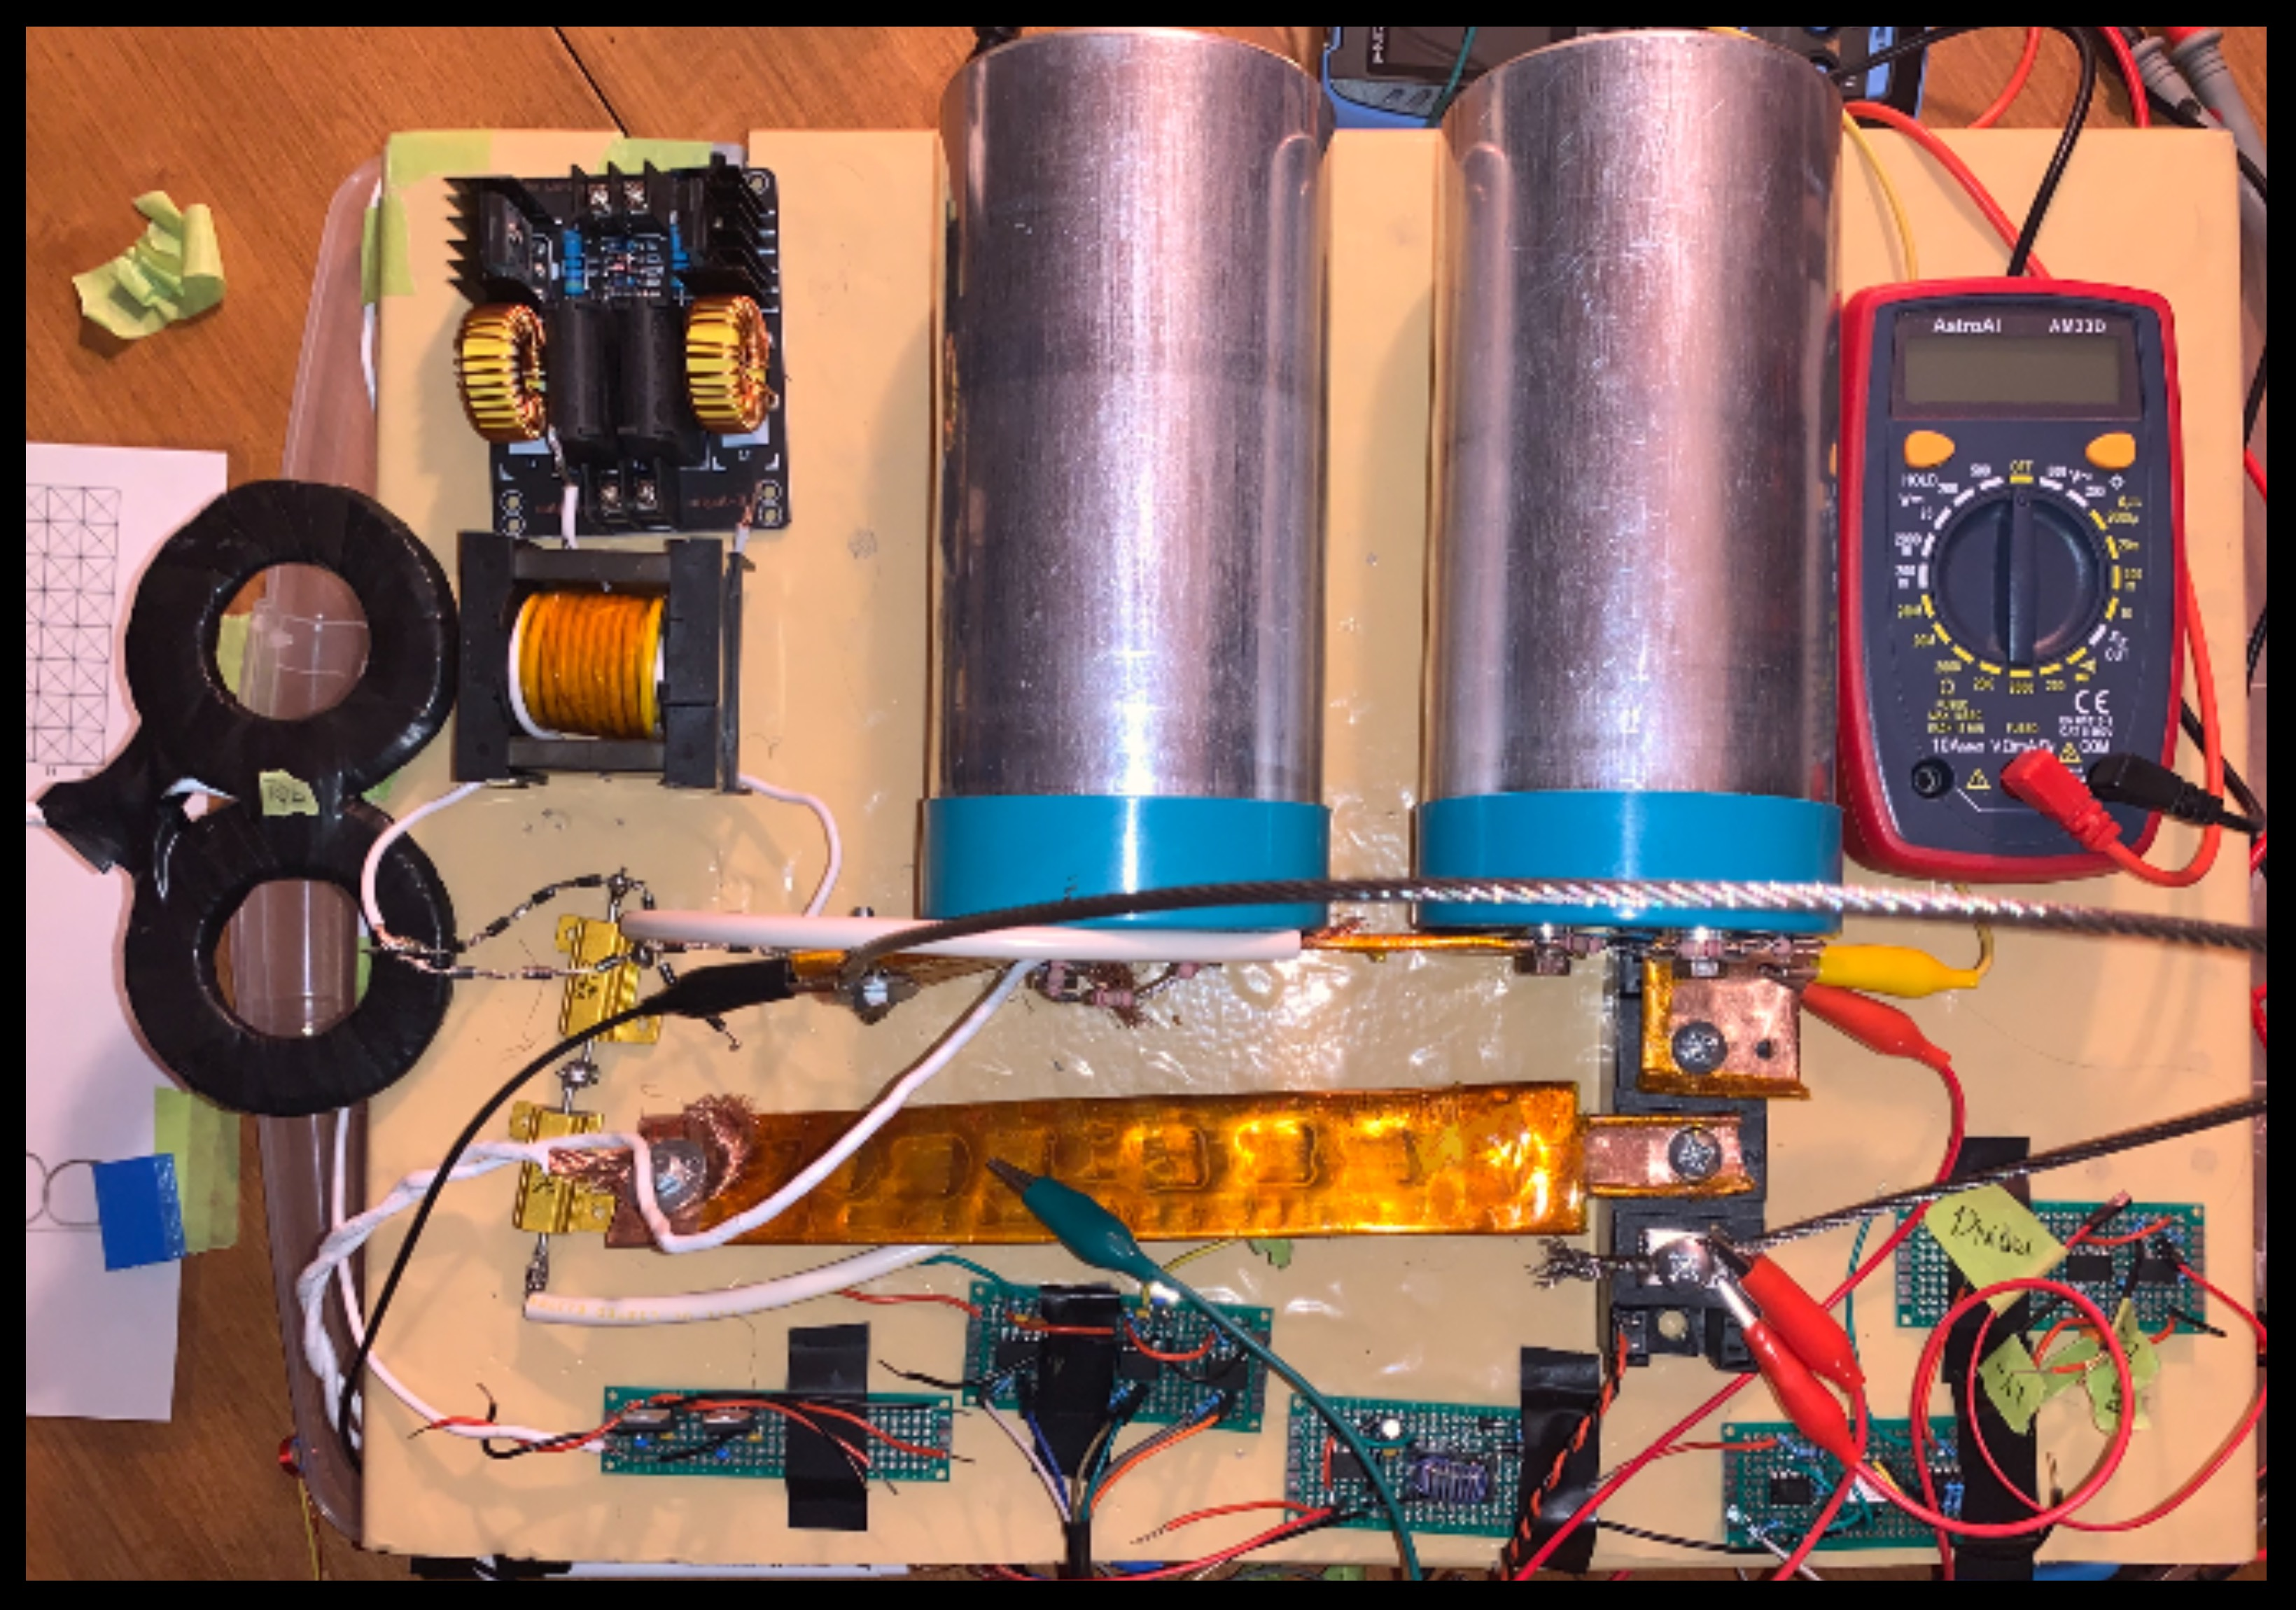
\includegraphics[width=\linewidth,height=23mm,keepaspectratio]{assets/history/mcgill-tms-prototype.jpg}
      \par{\tiny Prototype --- top view\par}\smallskip
      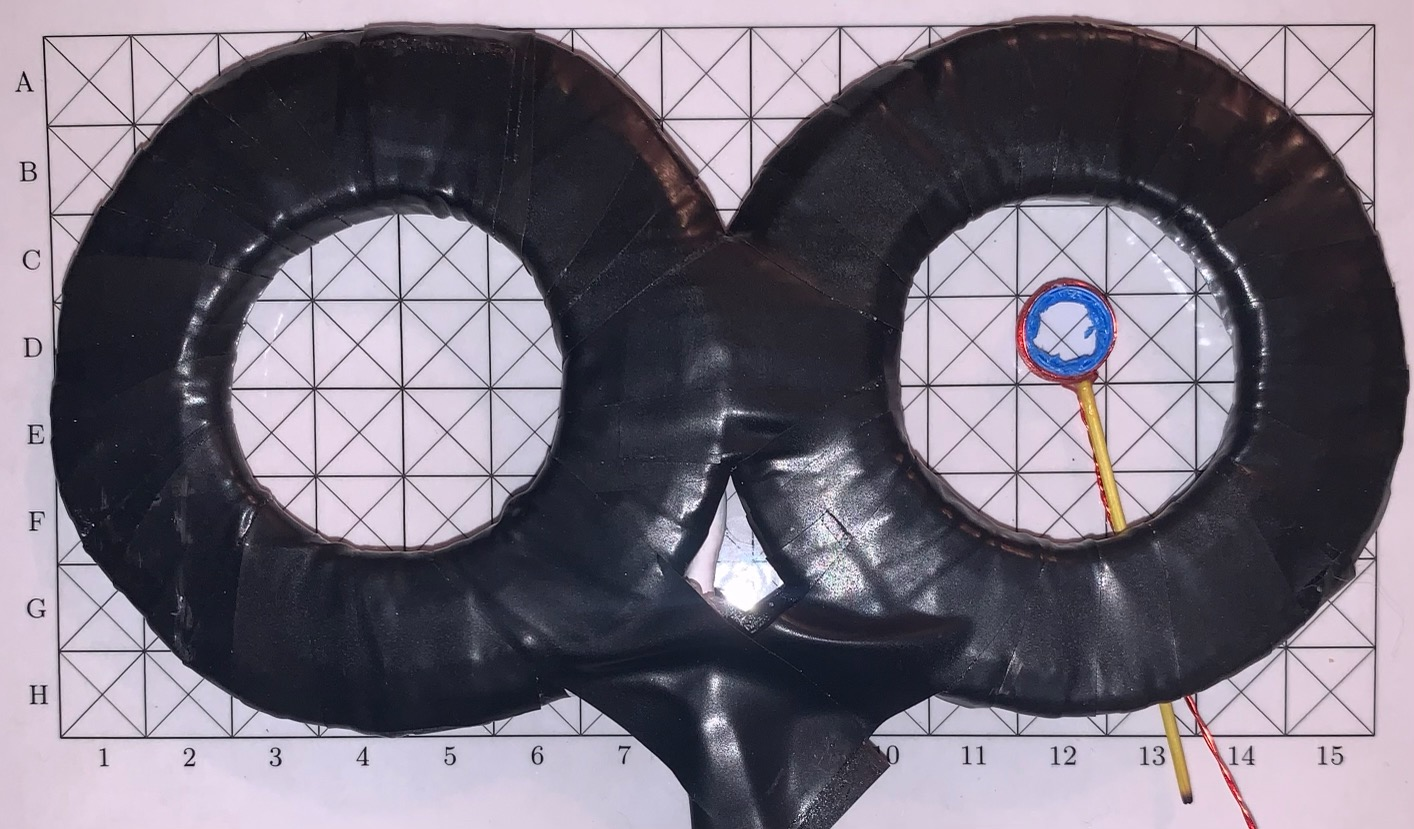
\includegraphics[width=\linewidth,height=21mm,keepaspectratio]{assets/history/mcgill-tms-coil.jpg}
      \par{\tiny Coil and field-measurement setup\par}
  \end{columns}
  {\tiny\color{NTXMuted}Sources: \href{https://www.linkedin.com/posts/maxence-lapatrie_brain-stimulation-research-can-be-expensive-activity-7498376586744709120-7w6N}{team announcement}; \href{https://doi.org/10.64898/2026.08.25.747050}{bioRxiv, August 2026}; photos: \href{https://www.mcgill.ca/ose/files/ose/2-35_-_maxence.pdf}{McGill project poster}\par}
  \note{[67:15--68:45] McGill NeuroTech announced the hardware team's new preprint. Credit Maxence Lapatrie, Yuzuha Isetani, Jathav Puvirajan, Antonella Catanzaro, Siqi Lyu, Han C. Nguyen, William Mathieu, and Milica Popovic. The preprint reports about USD700 in parts, excluding assumed bench equipment. Characterization combines measured magnetic fields with computational cortical-field estimates on an example anatomy; this is not evidence of demonstrated human stimulation or clinical efficacy. The announcement explicitly says the device is not approved for human stimulation or clinical use. High-energy electrical hardware requires qualified supervision and appropriate safety controls. Photos are extracted from the McGill-hosted project poster, not asserted to show the final preprint revision. Its earlier cost table differs from the new preprint; use the new preprint's rounded cost in the talk. The lesson is the scope of student engineering and characterization, not a DIY treatment recommendation.}
\end{frame}

\begin{frame}{More ambitious student projects: quantum sensors}
  \begin{columns}[c,onlytextwidth]
    \column{.51\textwidth}
      \small
  \NTXPoint{A starting point already exists}{Uncut Gem: an open-source diamond magnetometer from Quantum Village.}
  \NTXPoint{A student challenge}{Build the instrument, characterize its noise, and publish reproducible measurements.}
  \NTXPoint{A longer-term neurotech question}{What would it take to move from a magnetic-field demonstration to useful biosignal sensing?}
    \column{.45\textwidth}
      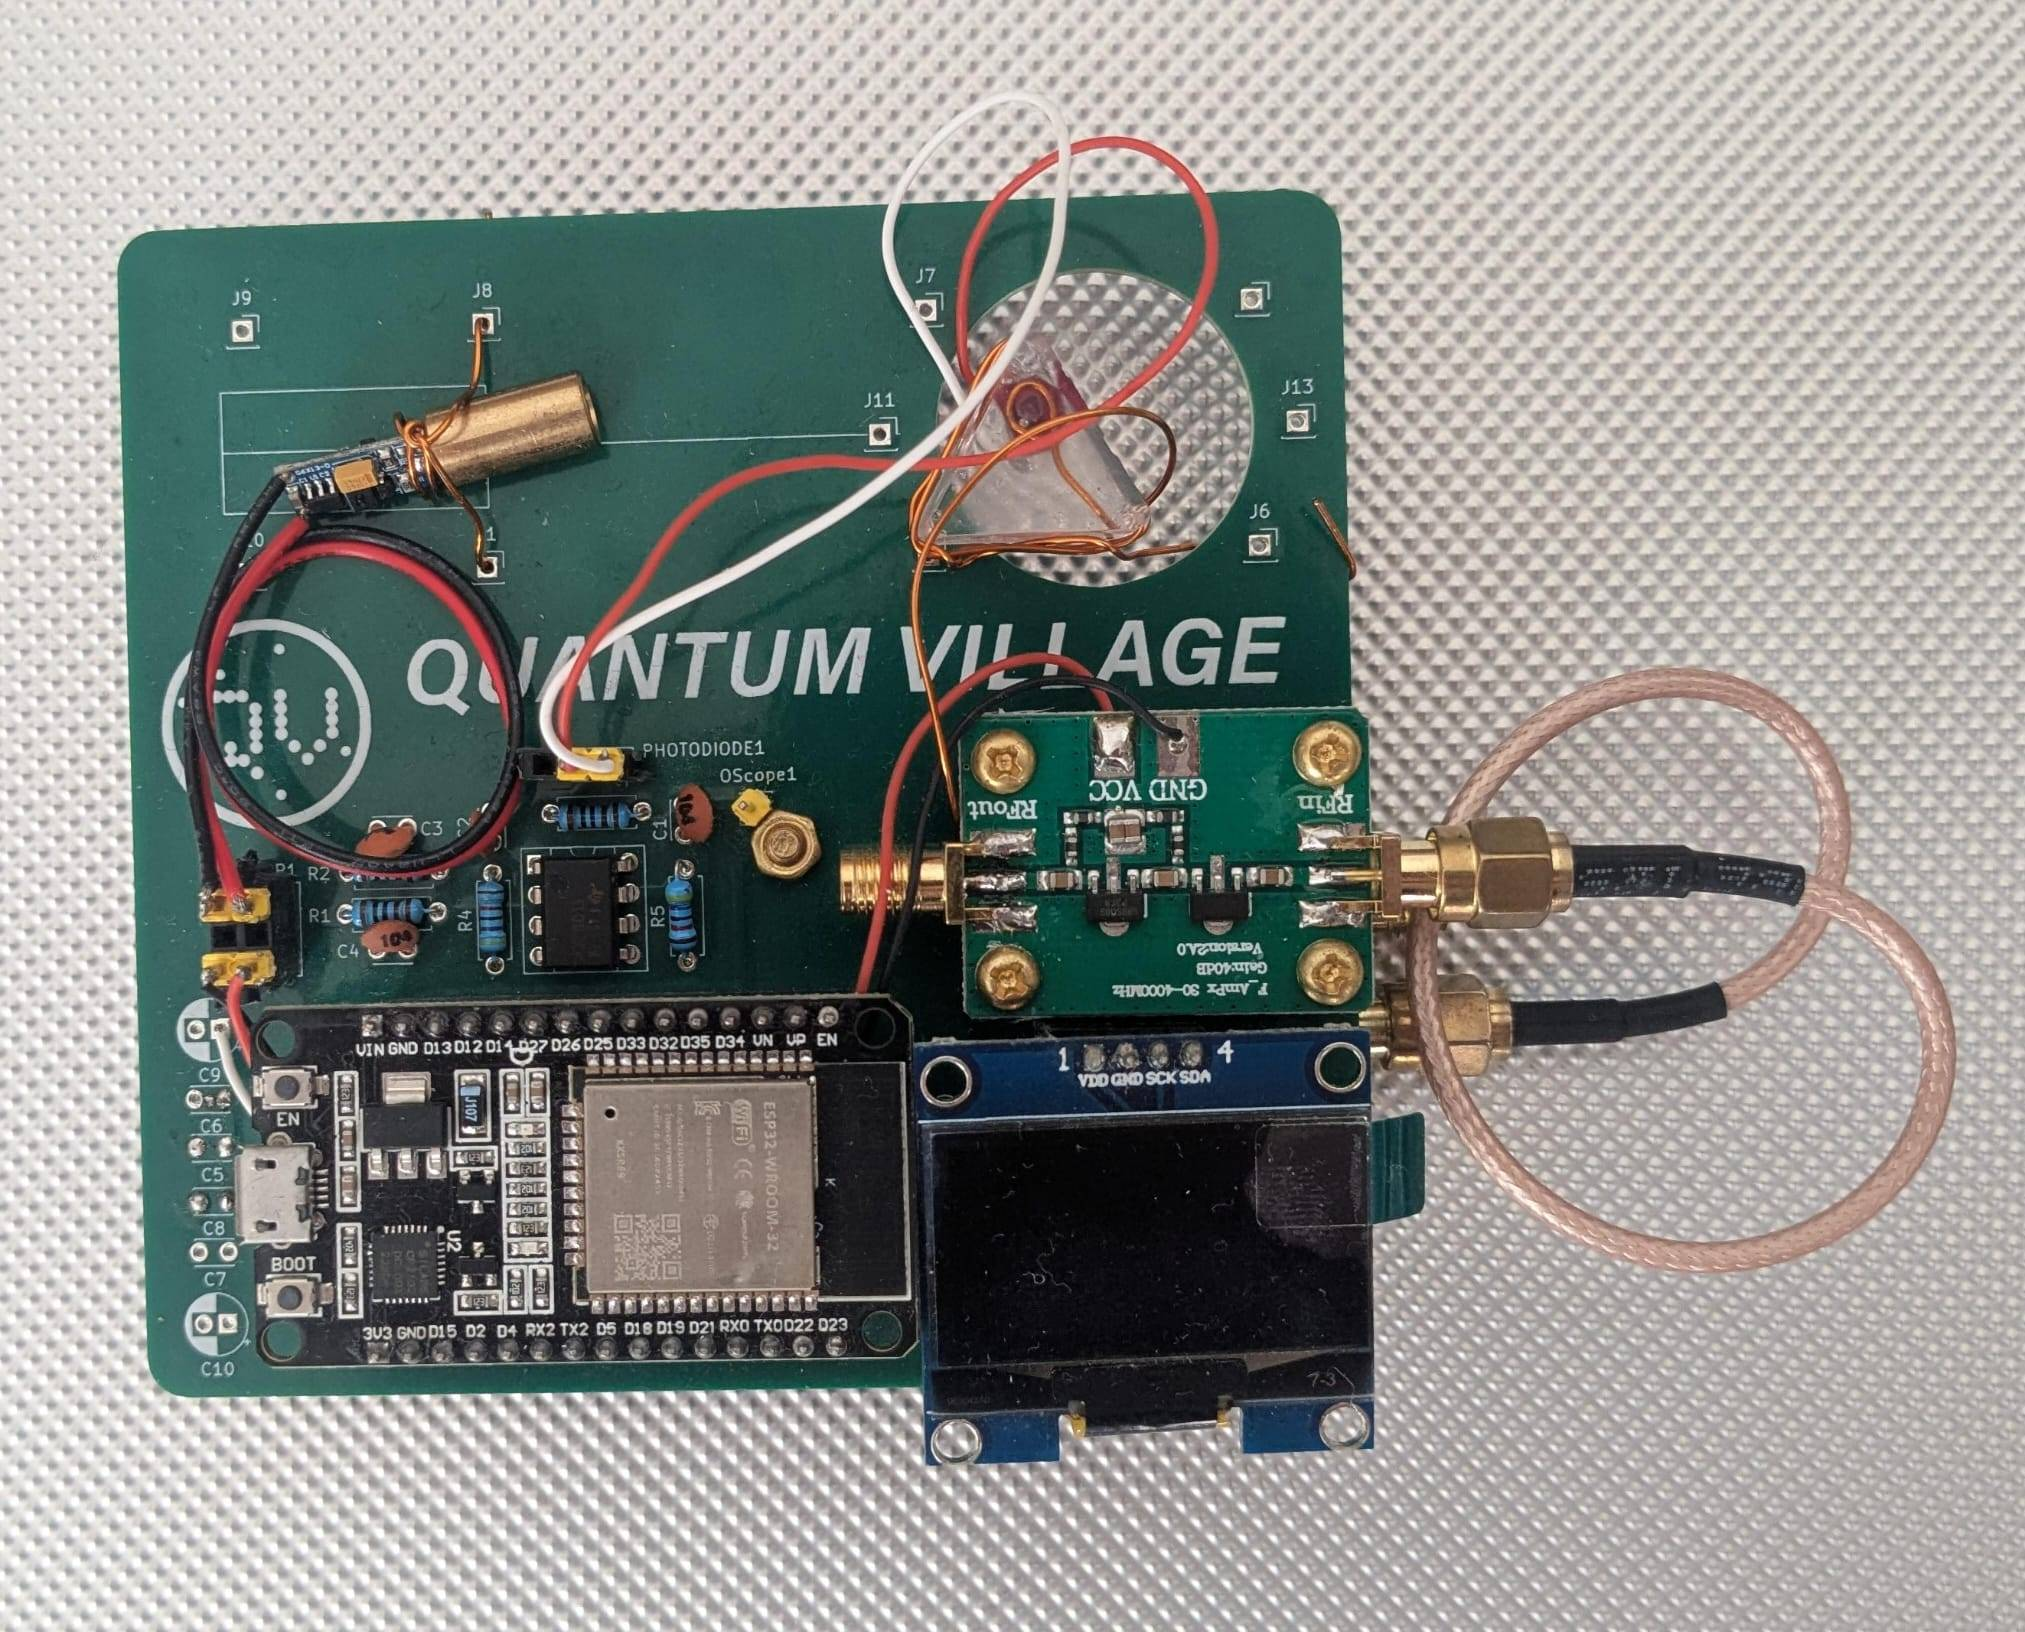
\includegraphics[width=\linewidth,height=45mm,keepaspectratio]{assets/history/uncut-gem-prototype.jpeg}\par\smallskip
      {\scriptsize Uncut Gem prototype\newline Photo: \href{https://quantumvillage.org/uncut-gem.html}{Quantum Village}\par}
  \end{columns}
  \NTXSource{https://arxiv.org/abs/2509.18329}{Carney and Kumaran: Uncut Gem; proposed student challenge, not an announced NTX program}
  \note{[68:45--70:15] Nitrogen-vacancy centers in diamond provide a concrete route into quantum sensing. The project publishes hardware and firmware. This is a learning platform, not a demonstrated brain scanner. Propose characterization and reproducibility as meaningful student contributions. Brain-field sensitivity is a separate research challenge; do not imply that assembling this kit produces an MEG instrument. Work requires appropriate equipment training and supervision.}
\end{frame}

\begin{frame}{Build an MRI: Johns Hopkins, September 16--18}
  \begin{columns}[c,onlytextwidth]
    \column{.50\textwidth}
      \small
  \NTXPoint{Coming up: DELTA DIY-MRI 2026}{Three days at Johns Hopkins University in Baltimore: learn, design, build, and scan.}
  \NTXPoint{A mentored, hands-on team project}{Build low-field MRI components and image a phantom: magnets, RF and gradient coils, acquisition, and reconstruction.}
  \NTXPoint{Free attendance; currently sold out}{Join the waitlist, or explore the public build resources and community.}
    \column{.46\textwidth}
      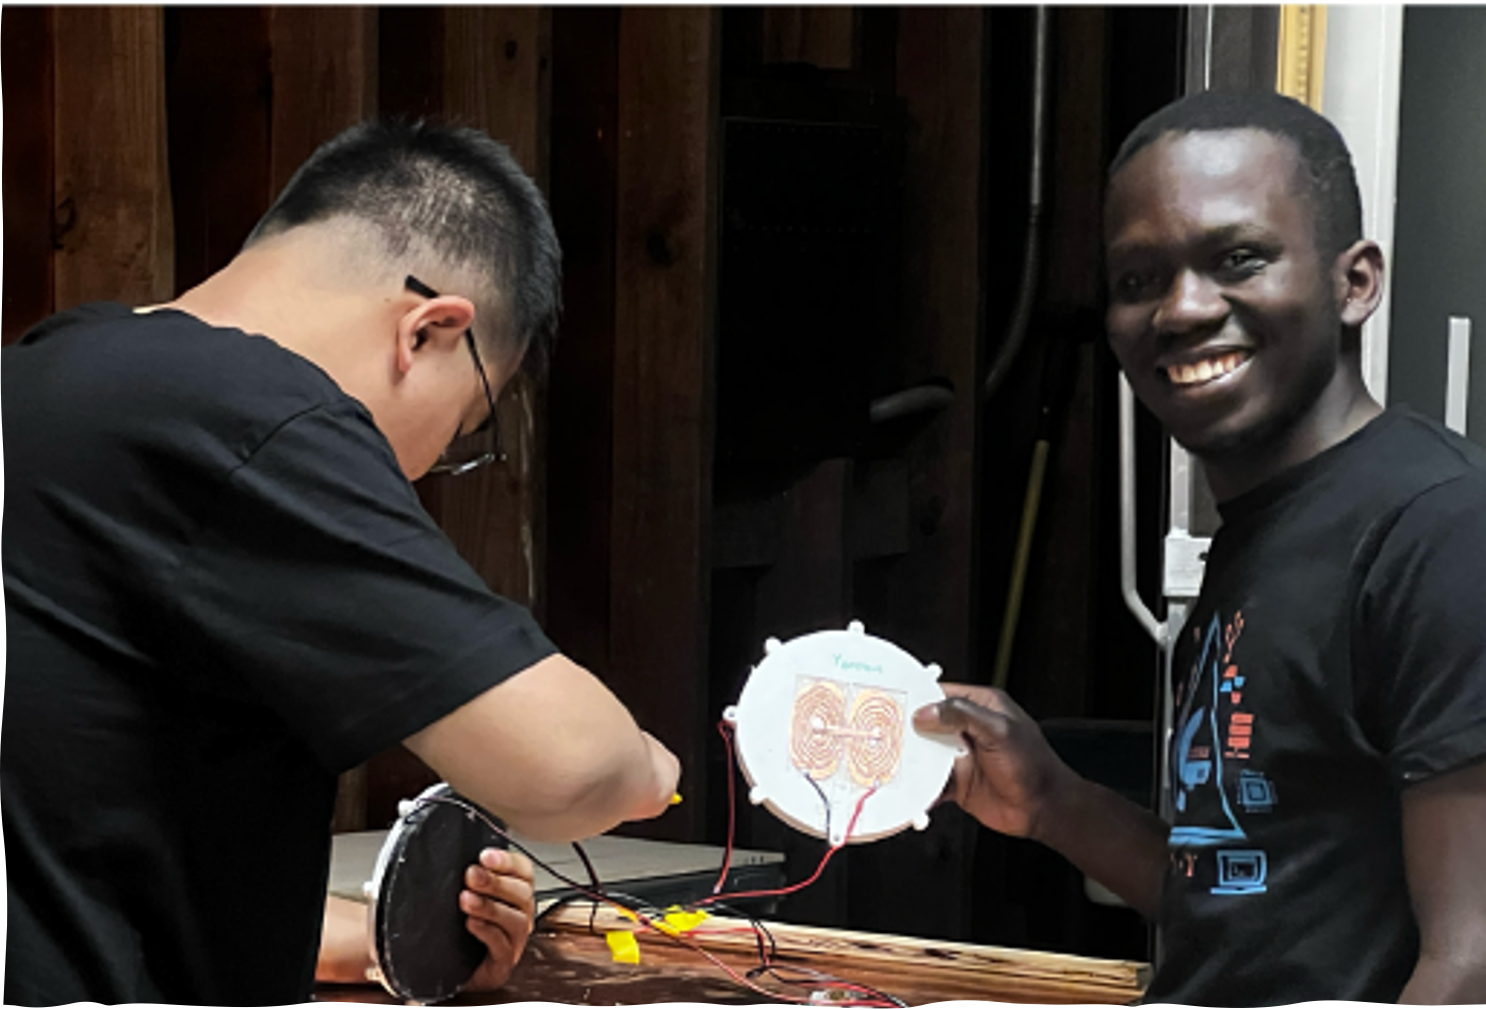
\includegraphics[width=\linewidth,height=42mm,keepaspectratio]{assets/history/jhu-diy-mri-build.png}\par\smallskip
      {\scriptsize Earlier workshop: hands-on building\newline Photo: DELTA DIY-MRI organizers\par}
  \end{columns}
  \NTXSource{https://delta-diy-mri.github.io/}{delta-diy-mri.github.io --- September 16--18, 2026; waitlist and resources}
  \note{[70:15--71:45] Announce the upcoming DELTA DIY-MRI workshop at Johns Hopkins University, Baltimore, September 16--18, 2026: nine days after this September 7 presentation. The official page checked September 6 says attendance is free but sold out, with a waitlist; do not promise a place. Its public wiki, repository and GitHub Discussions offer another route to participate. The picture is an earlier workshop photograph supplied on the organizer's site, not a photograph of the upcoming event. The previous event was May 5--7, 2025, not August 2026. This is an independent workshop, not an NTX-organized event. Mentored work covers magnet, RF, gradients, acquisition and reconstruction, ending in phantom imaging, not human scanning. The broader precedent remains MRI4ALL's four-day 2023 build. A student adaptation requires prepared components, expert mentors and magnet, RF, electrical and mechanical safety oversight.}
\end{frame}

\begin{frame}{LIBRE Hub: sharing an MRI build in Paraguay}
  \begin{columns}[T,onlytextwidth]
    \column{.62\textwidth}
      \NTXPoint{Open bioimaging across communities}{LIBRE Hub connects scientists, engineers, and makers in Latin America and beyond.}
      \NTXPoint{OSI2ONE in Asunci\'on}{Joshua Harper's team at Universidad Paraguayo Alemana described building an open low-field MRI.}
      \NTXPoint{Share what it takes to build}{Construction experience and practical considerations, presented in a June 2024 seminar.}
    \column{.32\textwidth}
      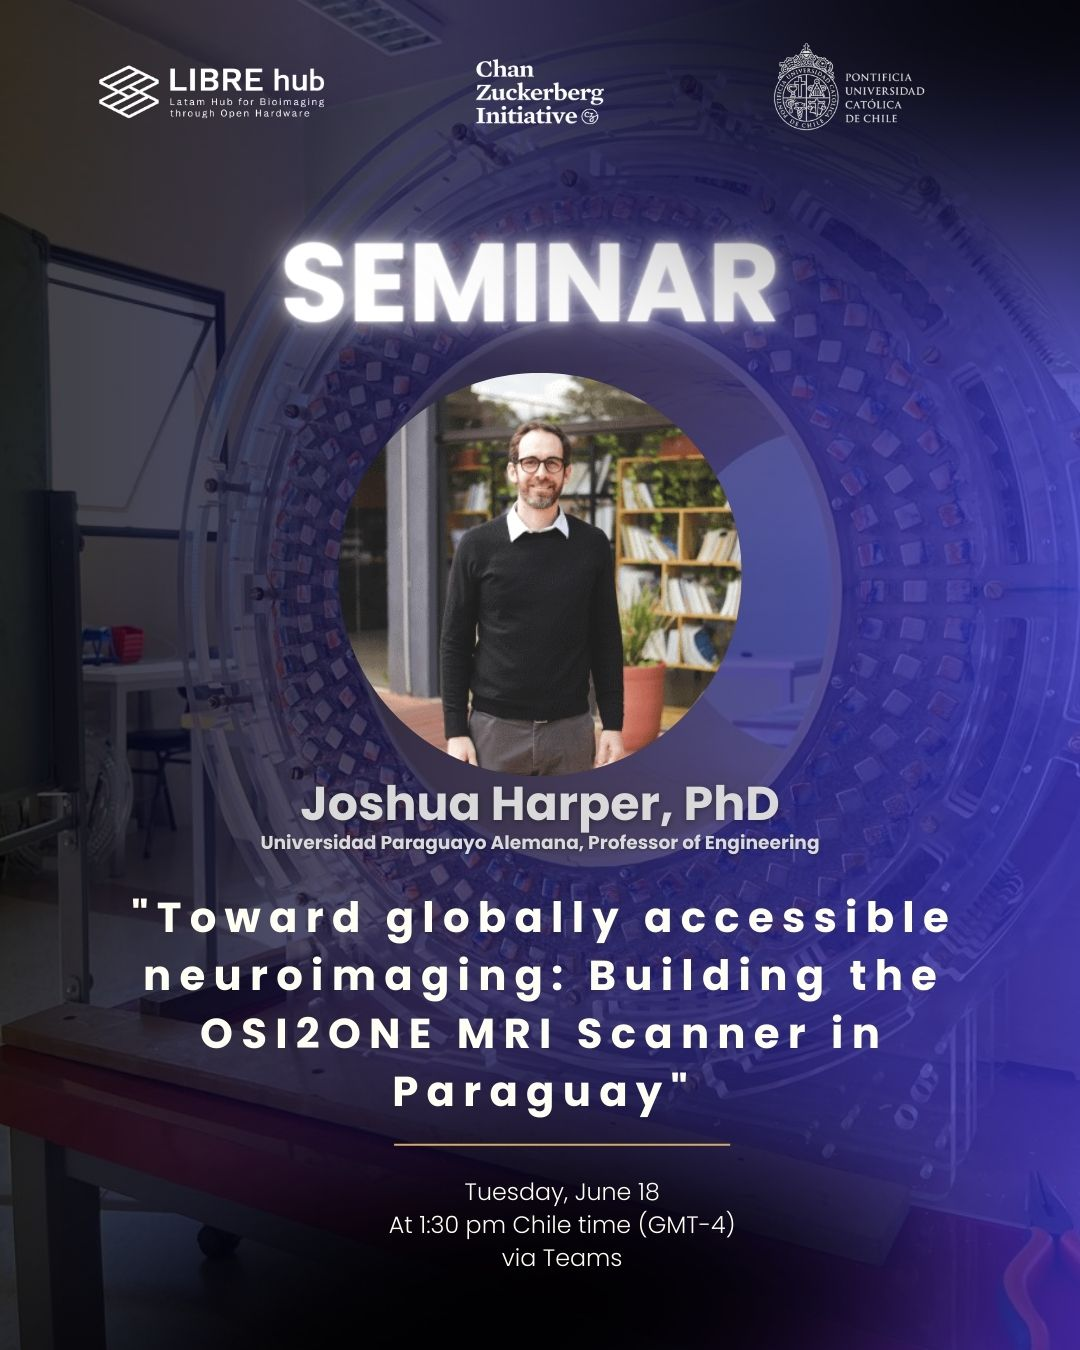
\includegraphics[width=\linewidth,height=49mm,keepaspectratio]{assets/history/librehub-paraguay-mri-2024.jpg}
      \par\smallskip{\scriptsize Original LIBRE Hub announcement\par}
  \end{columns}
  {\tiny\color{NTXMuted}Sources: \href{https://librehub.github.io/}{LIBRE Hub}; \href{https://librehub.github.io/2024/06/05/joshua-harper.html}{Joshua Harper seminar, 18 June 2024}; \href{https://youtu.be/NiABwvTVwp8}{recording}\par}
  \note{[71:45--73:15] LIBRE Hub is the dissemination and training community, not the builder or owner of this MRI project. The June 18, 2024 seminar describes a build underway at Universidad Paraguayo Alemana in Asuncion, Paraguay, using the Open Source Imaging Initiative's OSI2ONE design, intended for a neuroimaging project at a clinic in Bolivia. This source does not establish completed installation or clinical use in Bolivia. The image is the seminar flyer, not a documentary photograph of a completed Paraguayan scanner. Keep distinct from MRI4ALL's four-day build; no weekend completion claim is made for Paraguay. The lesson is locally developed expertise supported by shared designs and practical teaching.}
\end{frame}

\begin{frame}{CONNExIN: building expertise, looking toward Lagos}
  \begin{columns}[c,onlytextwidth]
    \column{.67\textwidth}
      \small
  \NTXPoint{Udunna Anazodo and the CONNExIN team}{Hybrid, hands-on neuroimaging training: developing local experts who can train others.}
  \NTXPoint{A shared contribution at ISMRM 2026}{Draper et al., abstract 563-01-002.\newline Morgan Hough, NeuroTechX --- co-author.}
  {\scriptsize\itshape Training 105 African clinicians and students in open neuroimaging analysis: CAMERA's dementia research program\par}
  \medskip
  \NTXPoint{Our hope for Lagos}{To become the first NeuroTechX city chapter in sub-Saharan Africa --- an ambition we hope to realize.}
    \column{.28\textwidth}
      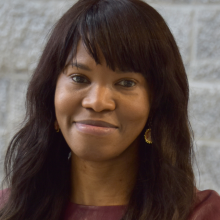
\includegraphics[width=\linewidth,height=35mm,keepaspectratio]{assets/people/udunna-anazodo.png}\par\smallskip
      {\small Udunna Anazodo\par}
      {\tiny Portrait: \href{https://mcmedhacks.com/team/dr-udunna-anazodo/}{McMedHacks}\par}
  \end{columns}
  {\tiny\color{NTXMuted}Sources: \href{https://event.fourwaves.com/connexin/pages/41f08c9e-6502-46b4-bf53-ec5a6cf095b7}{CONNExIN program}; \href{https://echo.ismrm.org/abstracts/view/a98f4909-2b73-49d0-849b-14f932d68bca}{ISMRM 2026 abstract}; Lagos aspiration: Morgan Hough\par}
  \note{[73:15--74:45] The official program spelling is CONNExIN. Credit Udunna Anazodo and the whole team. Its organizers describe a free hybrid train-the-trainer initiative connecting the MiND Lab at the Montreal Neurological Institute with McGill's aging research centre, the Medical Artificial Intelligence Lab in Nigeria, and CAMERA. Team-based learning builds local neuroimaging expertise. The 2025 program lists the MAI Lab in Lagos as its hybrid location. The accepted ISMRM 2026 digital-poster abstract is Training 105 African clinicians and students in open neuroimaging analysis: CAMERA's dementia research program, presented by Ethan Draper in Cape Town on May 13. Morgan is listed as a co-author with NeuroTechX affiliation. The title's 105 is not independently verified as a completion or certification count: the full abstract and results are access-restricted and were not read. Our hope is for Lagos to become the first NTX city chapter in sub-Saharan Africa. This is Morgan's aspiration, not a claim that a chapter has launched or an independently audited first-ever ranking. The public NTX directory mentions Lagos without proving launch status. Do not conflate this with the existing ISMRM African Chapter or imply that NTX owns CONNExIN.}
\end{frame}


\begin{frame}{From making almost anything to growing almost anything}
  \begin{columns}[c,onlytextwidth]
    \column{.66\textwidth}
      \small
      \setlength{\medskipamount}{3pt}
      \NTXPoint{1998 --- How to Make (Almost) Anything}{Neil Gershenfeld's MIT course: learn fabrication by building.}
      \NTXPoint{2001 onward --- CBA / Fab Labs}{Center for Bits and Atoms: information meets fabrication. Fab Labs share tools; Fab Academy connects local learning.}
      \NTXPoint{2015 --- How to Grow (Almost) Anything}{Distributed synthetic biology education through Fab Labs and community biology labs.}
      \NTXPoint{2019 / 2021 --- Campus to global classrooms}{MIT/Harvard offering in 2019; remote experiments, robotics, and mentoring in the 2021 redesign.}
    \column{.30\textwidth}
      \centering
      
\includegraphics[width=\linewidth,height=23mm,keepaspectratio]{assets/history/cba-official-logo.jpg}
      \par\bigskip
      
\includegraphics[width=\linewidth,height=19mm,keepaspectratio]{assets/history/htgaa-logo.pdf}
      \par\smallskip{\scriptsize How to Grow (Almost) Anything\par}
  \end{columns}
  {\tiny\color{NTXMuted}Sources: \href{https://betterworld.mit.edu/spectrum/issues/spring-2018/how-to-make-almost-anything-better/}{MIT: HTMAA}; \href{https://cba.mit.edu/about/}{CBA}; \href{https://fabfoundation.org/getting-started/}{Fab Foundation}; \href{https://www.media.mit.edu/articles/a-global-lab-for-teaching-and-practicing-synthetic-biology/}{MIT: HTGAA history}\par}
  \note{[74:45--76:15] MIT's official course name is How to Make (Almost) Anything, abbreviated HTMAA, rather than HTBAA. Gershenfeld began it in 1998. CBA launched with NSF support in 2001, studying the relationship between information and physical things. Fab Labs extend access to fabrication tools; Fab Academy distributes instruction across local labs. These are related, not interchangeable institutions. HTGAA began globally in 2015, drawing on the Fab Lab and community biology networks. David Kong and George Church offered it to MIT and Harvard graduate students in 2019; Joseph Jacobson is also credited as an instructor. In 2021, remote robotic experiments and mentoring supported distributed participation. The connection to Biopunk Lab here is the community-learning model, not a claim of formal MIT, Fab Lab, or HTGAA affiliation.}
\end{frame}

\begin{frame}{From using chips to learning how to make them}
  \begin{columns}[c,onlytextwidth]
    \column{.47\textwidth}
      \small
      \NTXPoint{Hacker Fab: open fabrication}{Student-built tools, shared processes, and device characterization.}
      \NTXPoint{Demonstrated at CMU}{Working transistors, including self-aligned NMOS devices.}
      \NTXPoint{Our next ambition}{Explore CMOS access and custom sensor electronics through fabrication communities.}
    \column{.49\textwidth}
      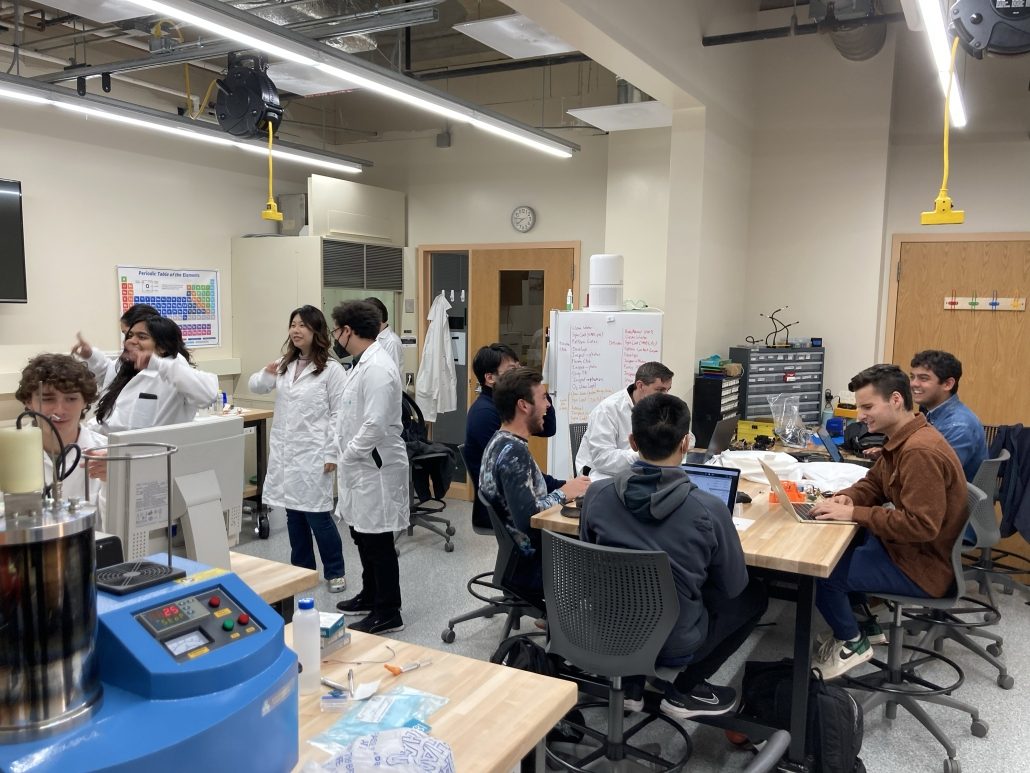
\includegraphics[width=\linewidth,height=45mm,keepaspectratio]{assets/history/hackerfab-cmu-lab.jpg}
      \par\smallskip{\scriptsize Inside Hacker Fab at Carnegie Mellon\par}
  \end{columns}
  \NTXSource{https://hackerfab.ece.cmu.edu/}{Hacker Fab at Carnegie Mellon University; CMOS access is a proposed direction}
  \note{[76:15--77:45] Hacker Fab started at CMU in 2023. Its documented NMOS demonstration should not be relabeled as a complete CMOS process or a commercial foundry service. The relevant lesson is access to tools and process knowledge. For neurotech students, projects could span test structures, characterization, and sensor-interface designs as facilities allow. No partnership or fabrication access is promised. Semiconductor processing requires facility-specific chemical, vacuum, thermal, and electrical safety training.}
\end{frame}

\begin{frame}{Biopunk Lab: a home for synthetic neurobiology}
  \begin{columns}[c,onlytextwidth]
    \column{.49\textwidth}
      \small
      \NTXPoint{Back in San Francisco}{Founding Member of Biopunk Lab, working on synthetic neurobiology.}
      \NTXPoint{A place for hands-on work}{Cell culture facility for Neurotech@Berkeley's wetware group.}
      \NTXPoint{Community enables experiments}{Supporting replication work inspired by Mind in Vitro and DishBrain research.}
    \column{.47\textwidth}
      \centering
      
\includegraphics[height=17mm]{assets/history/biopunk-logo.png}
      \par\medskip
      \begin{minipage}[c]{.40\linewidth}
        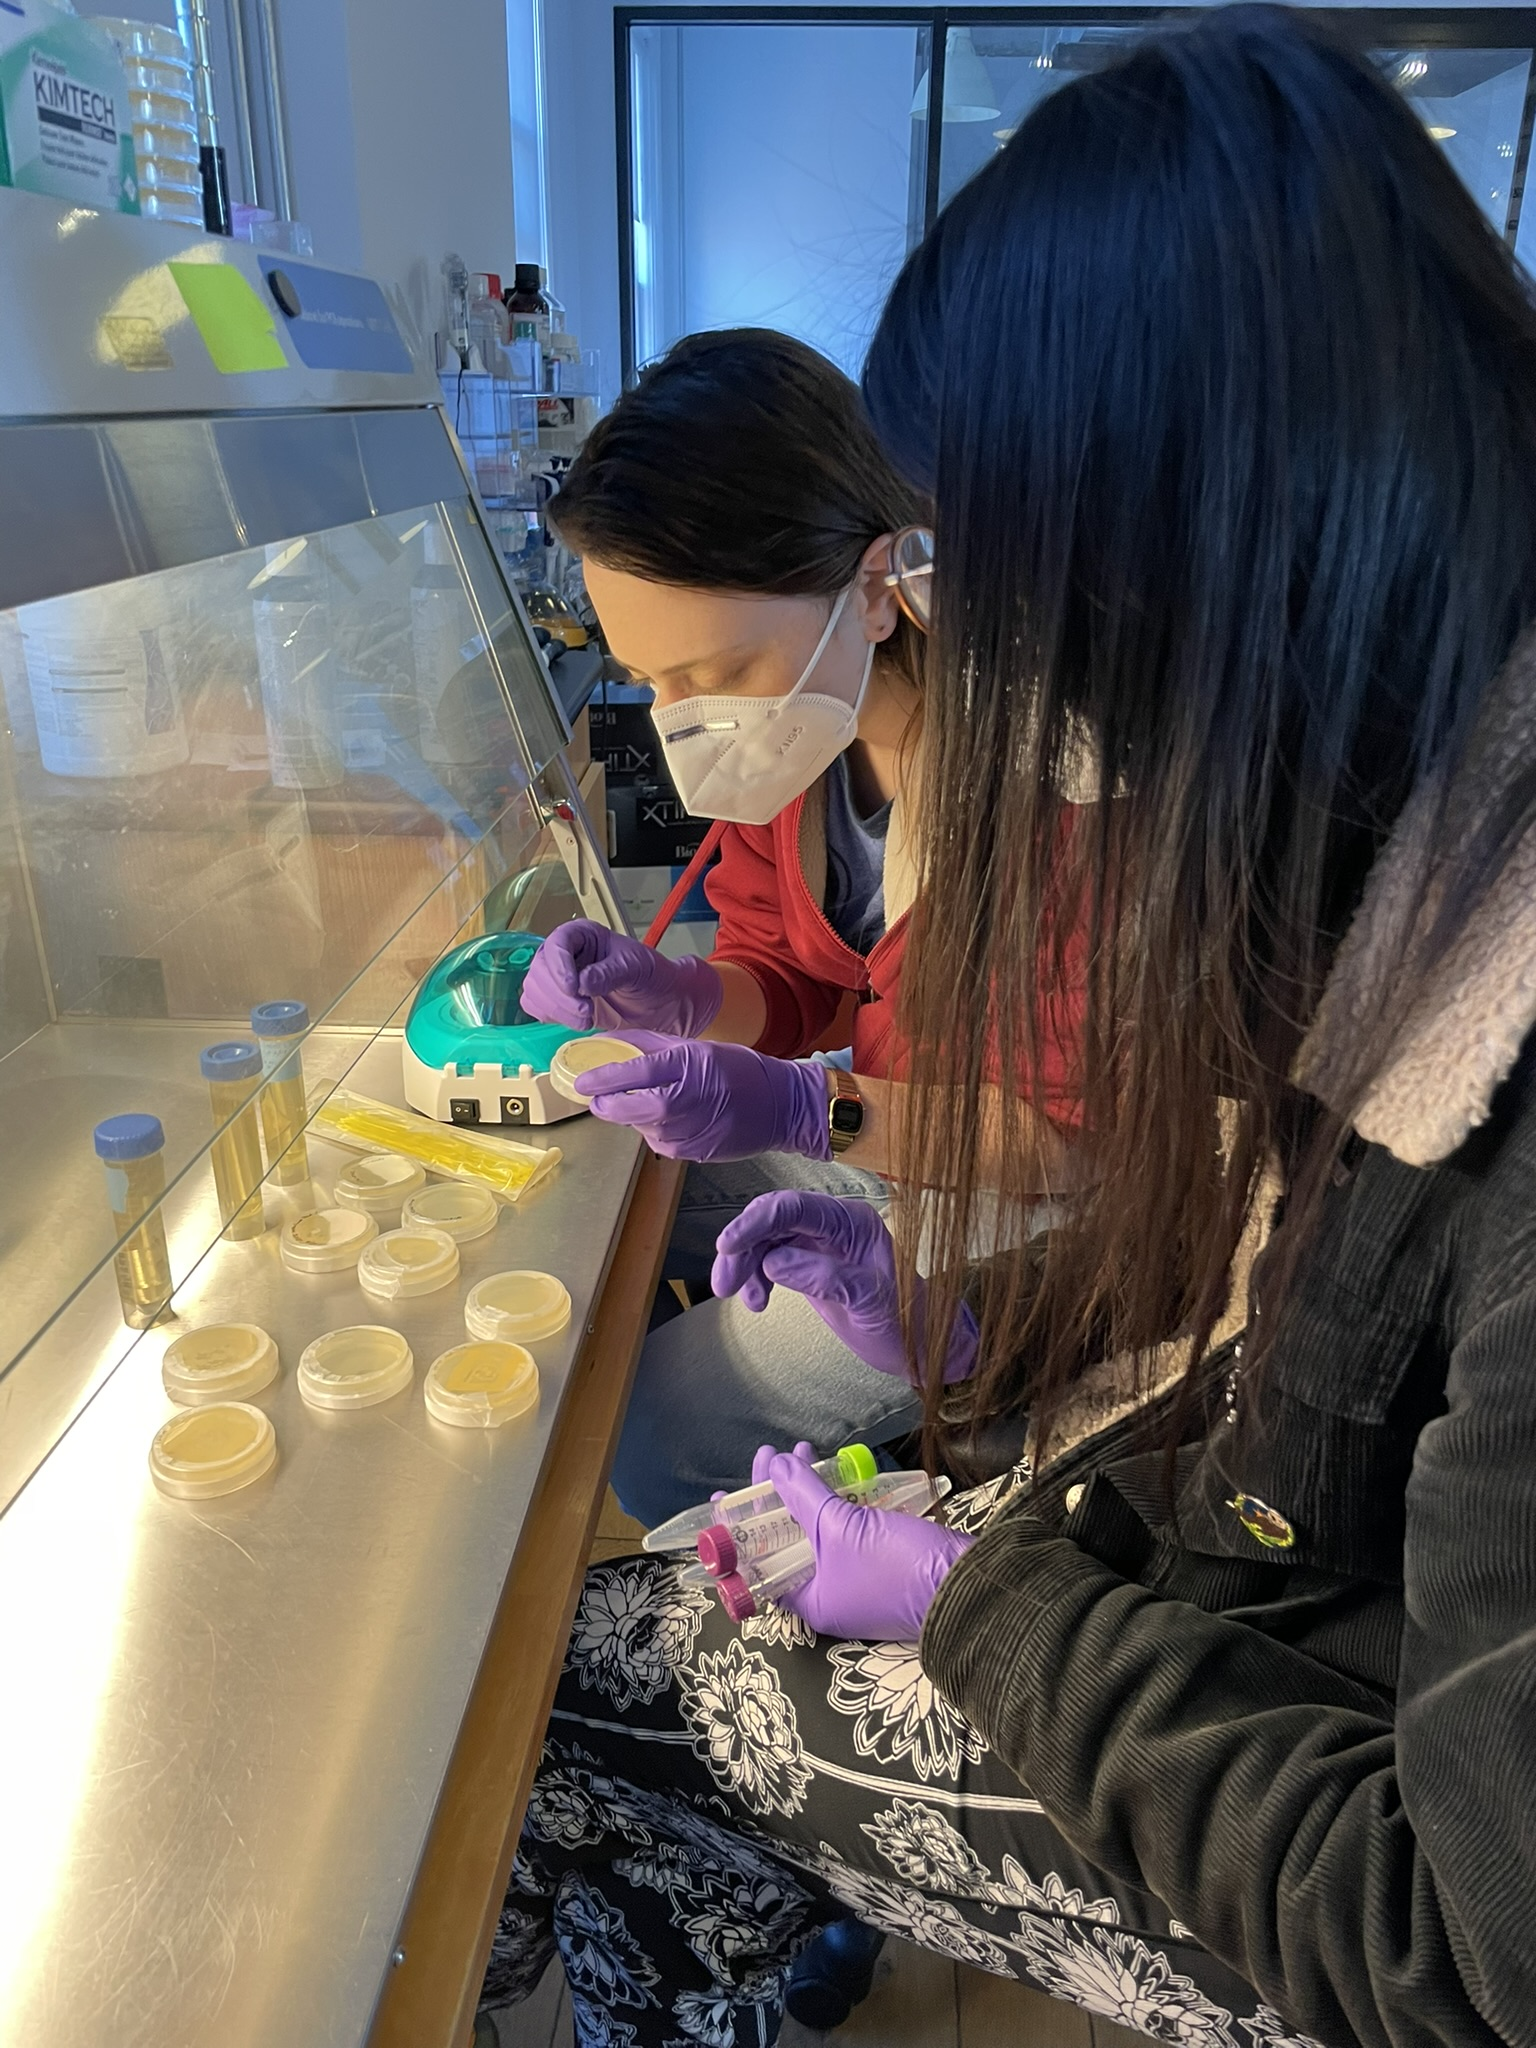
\includegraphics[width=\linewidth,height=31mm,keepaspectratio]{assets/history/biopunk-biosafety.jpeg}
      \end{minipage}\hfill
      \begin{minipage}[c]{.57\linewidth}
        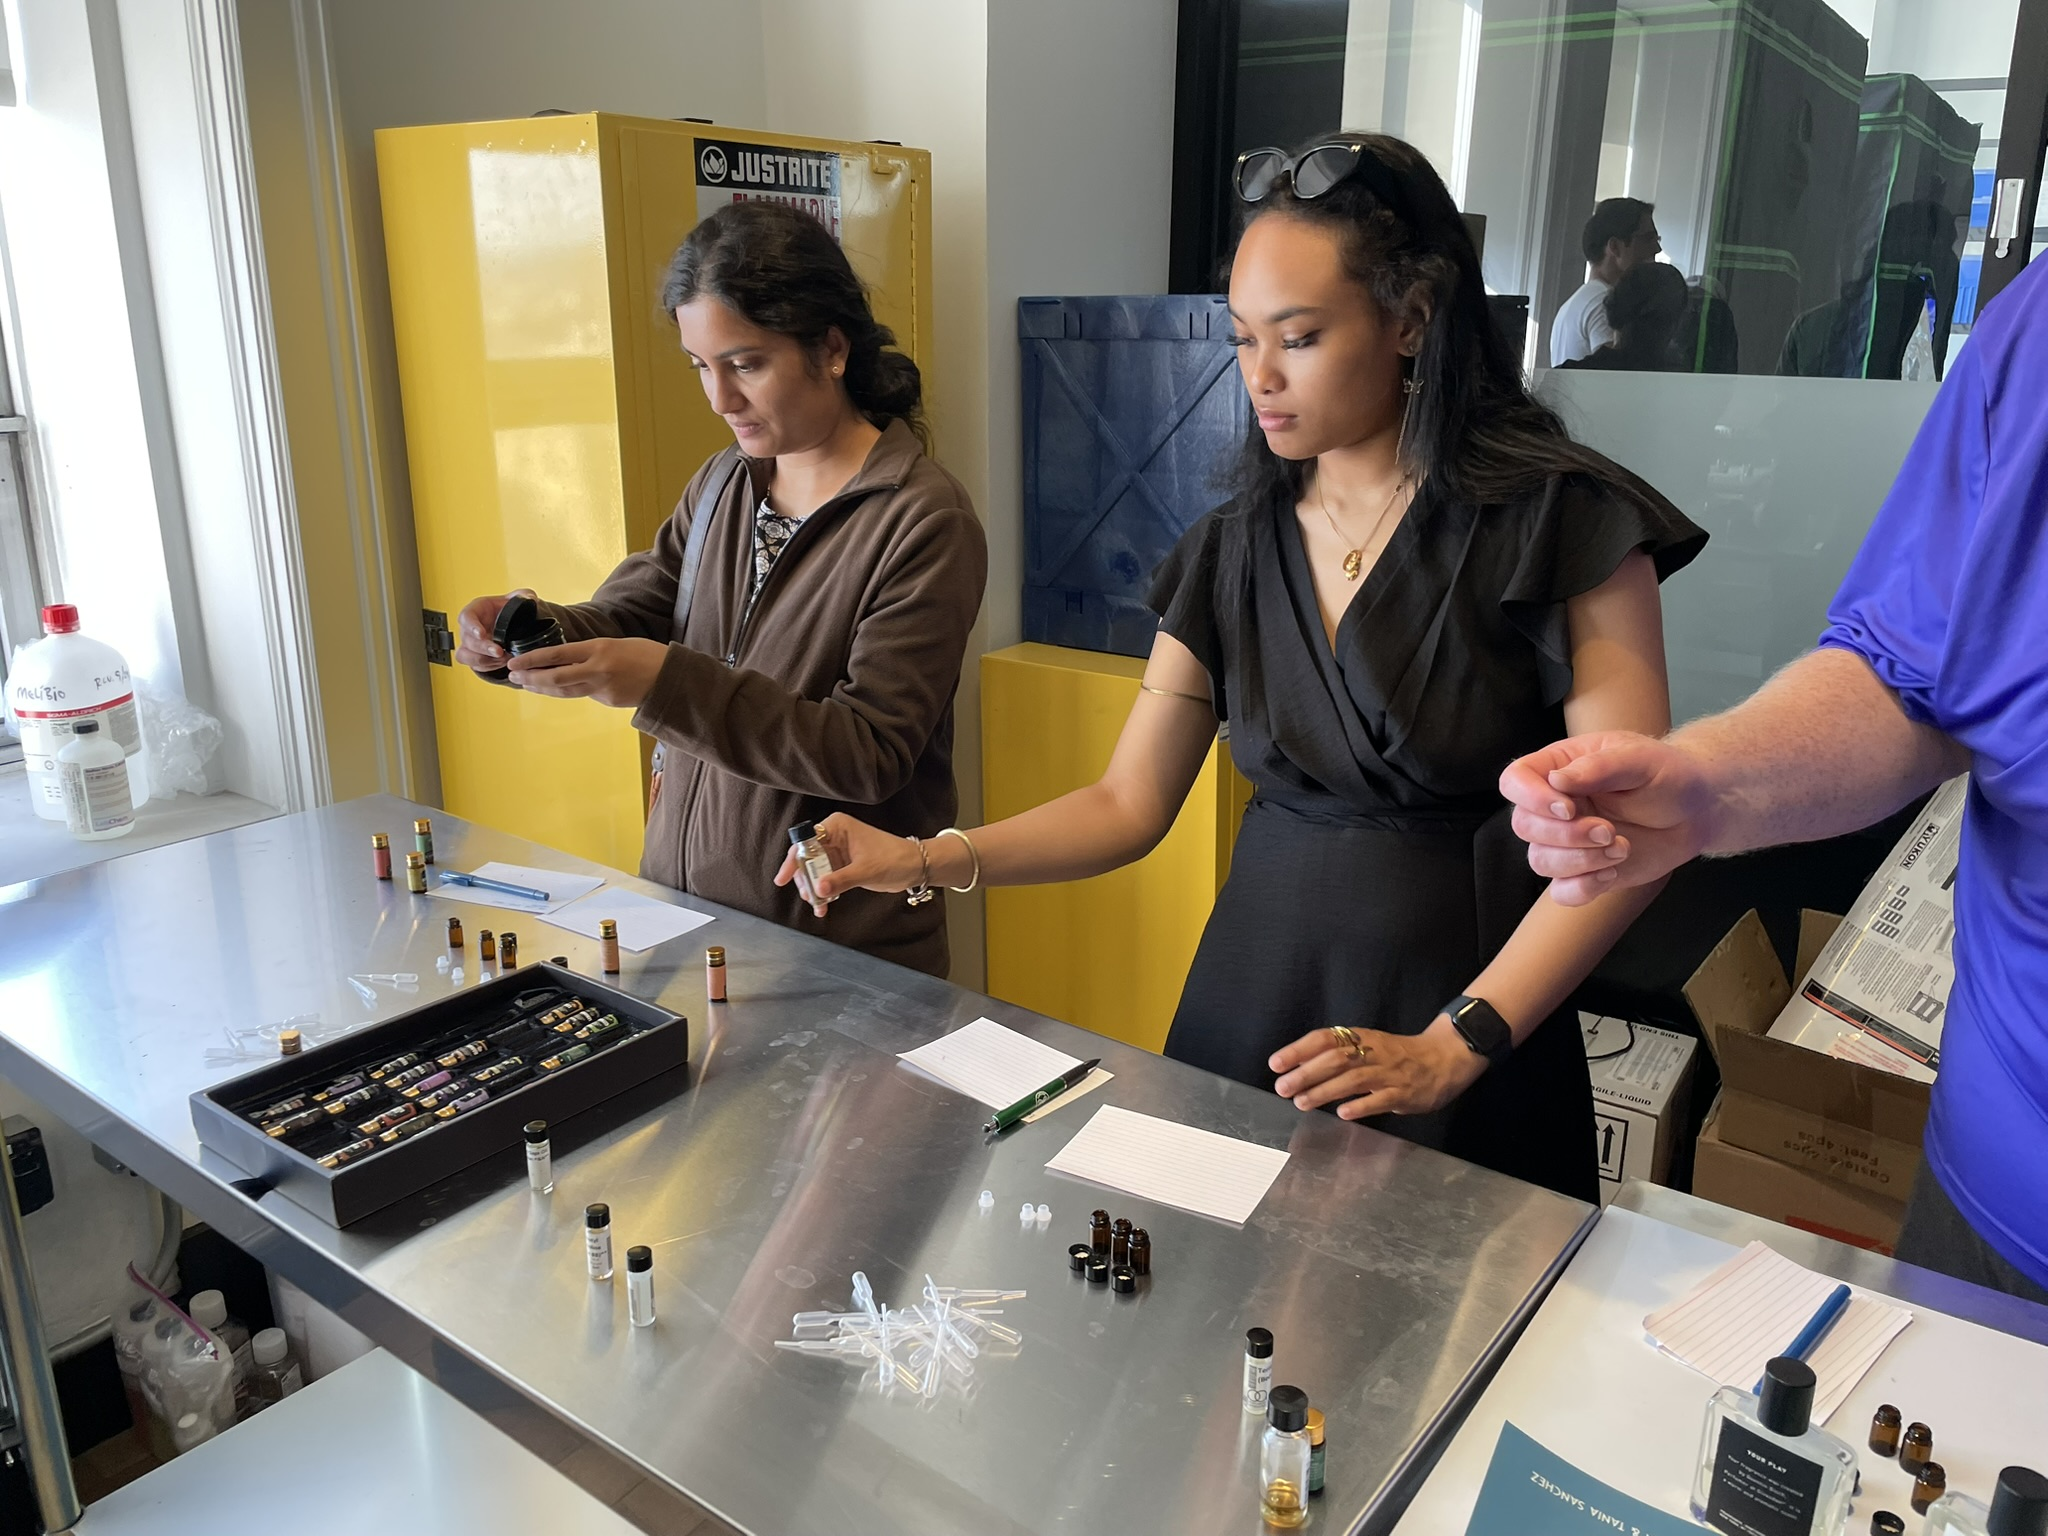
\includegraphics[width=\linewidth,height=31mm,keepaspectratio]{assets/history/biopunk-workshop.jpeg}
      \end{minipage}
      \par\smallskip{\scriptsize Lab work and community workshop\par}
  \end{columns}
  {\tiny\color{NTXMuted}Activities: Morgan Hough's firsthand account. Photos and logo: \href{https://biopunklab.com/}{Biopunk Lab}\par}
  \note{[77:45--79:15] Introduce Biopunk Lab through your experience as a founding member working on synthetic neurobiology. You report that Neurotech@Berkeley's wetware group currently uses the lab as its cell culture facility. This is a firsthand account, not an independently verified institutional announcement. The next slide distinguishes the Illinois Mind in Vitro hardware from Cortical Labs' DishBrain experiments and introduces the Open Ephys collaboration. Describe the work as an effort toward replication, not a completed replication or demonstrated learning result. Cell provenance, biosafety, and ethical oversight remain essential.}
\end{frame}

\begin{frame}{The future of neurobiotech: community wetware}
  \centering
  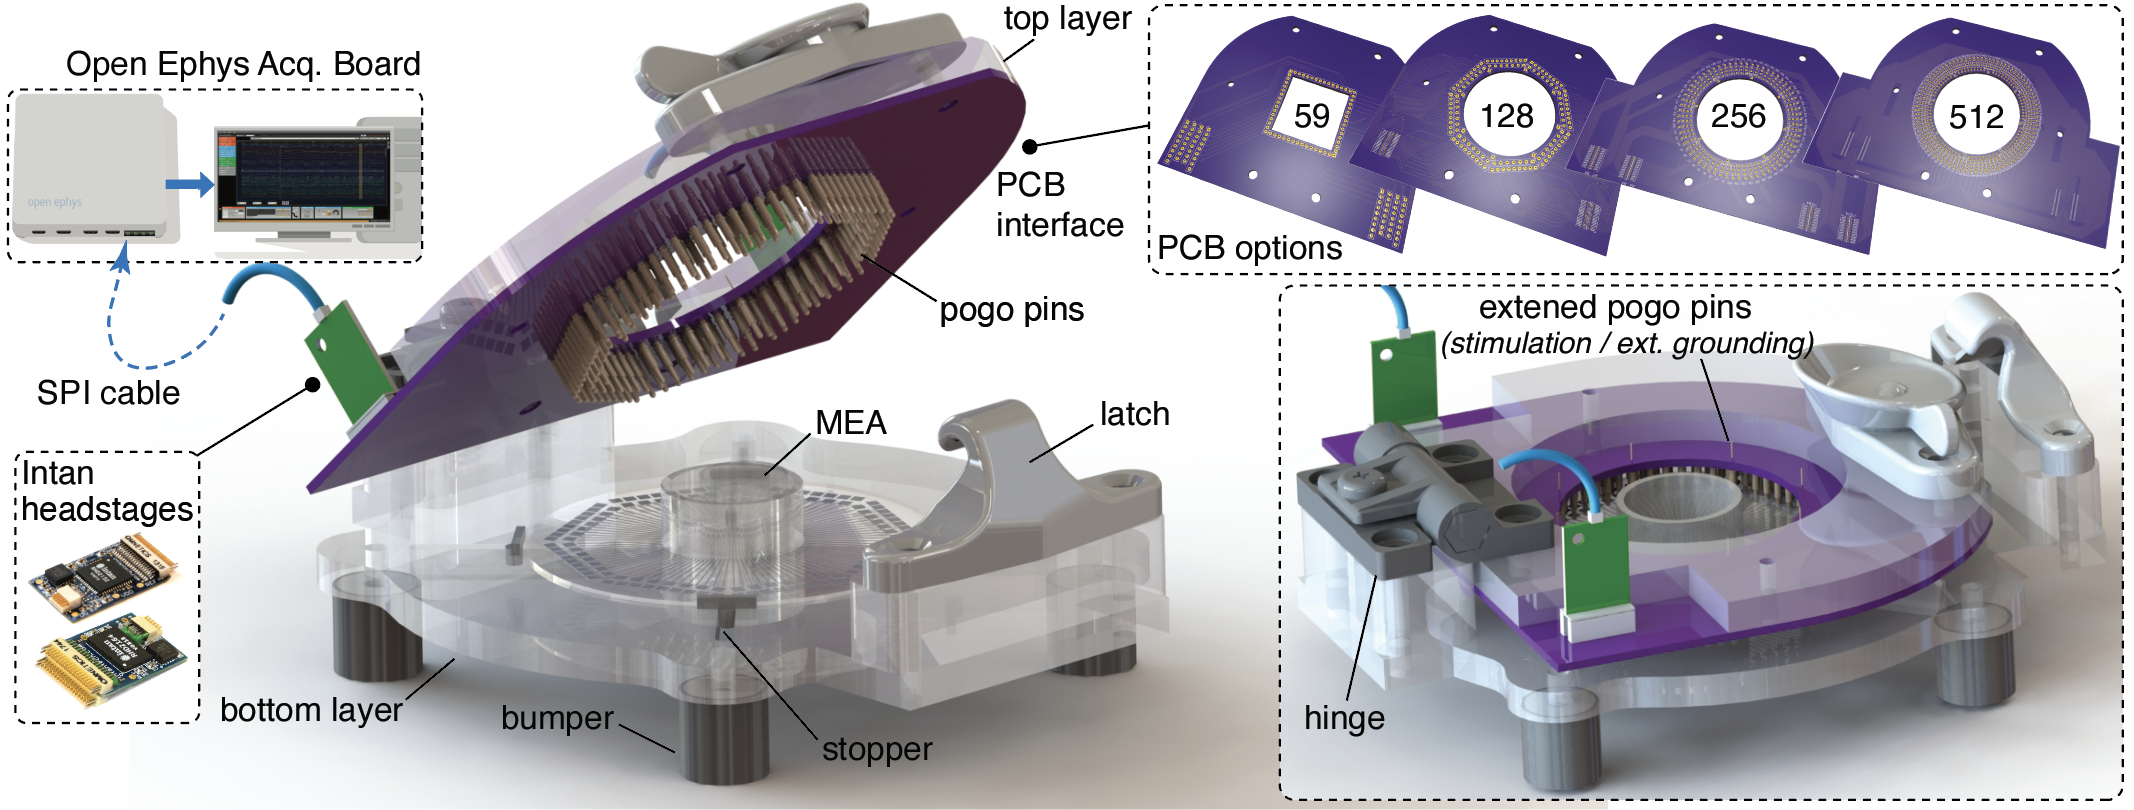
\includegraphics[width=.91\linewidth,height=28mm,keepaspectratio]{assets/history/mind-in-vitro-overview.jpg}
  \par\smallskip
  \raggedright
  {\small
  \textbf{Mind in Vitro as a starting point} --- Open hardware for interfacing with living neurons.\par\smallskip
  \textbf{Working with Open Ephys} --- Developing a low-cost MEA/bioreactor for neuronal stimulation and recording.\par\smallskip
  \textbf{Neurotech@Berkeley wetware at Biopunk Lab} --- Using the cell-culture facility to pursue replication, guided by DishBrain and follow-up studies.\par}
  \medskip
  {\tiny\color{NTXMuted}Image: \href{https://gazzolalab.github.io/MiV-OH/overview/system_overview.html}{MiV-OH / Gazzola Lab}; \href{https://doi.org/10.1002/advs.202306826}{Zhang et al., 2024}; \href{https://doi.org/10.1016/j.neuron.2022.09.001}{DishBrain, 2022}; local work: Morgan Hough\par}
  \note{[79:15--81:15] Morgan reports collaboration with Open Ephys toward a low-cost MEA/bioreactor and Berkeley wetware's current use of Biopunk Lab for cell culture. These are firsthand accounts, not independently verified institutional announcements. The image is the Illinois MiV design, not a completed local device. MiV uses custom MEAs, Intan headstages, Open Ephys acquisition, and modular stimulation/fluidic interfaces. DishBrain (Kagan et al., Neuron 2022) uses a different high-density MEA platform for closed-loop Pong experiments. Follow-ups: Habibollahi et al., Nature Communications 2023, on critical dynamics; Khajehnejad et al., 2024 preprint arXiv:2405.16946, on sample efficiency. Full citations are in assets/history/mind-in-vitro-sources.md. Hardware replication is distinct from reproducing behavioral results; no completed Berkeley replication, learning, or sentience result is claimed. Appropriate cell provenance, biosafety, and ethical oversight remain necessary.}
\end{frame}

\begin{frame}{Marley Xiong and collaborators: projects to Aleph}
  \begin{columns}[c,onlytextwidth]
    \column{.49\textwidth}
      \small
      \NTXPoint{Student community: McGill NeuroTech}{Marley Xiong, Raffi Hotter, and fellow students: Milo, NTX competition 2019.}
      \NTXPoint{Brainhack: testing a difficult idea}{A ten-day acoustoelectric tank proof of concept with collaborators.}
      \NTXPoint{Aleph: continuing the ambition}{Marley, Raffi, and Lev Chizhov: announced cofounders.}
    \column{.47\textwidth}
      \centering
      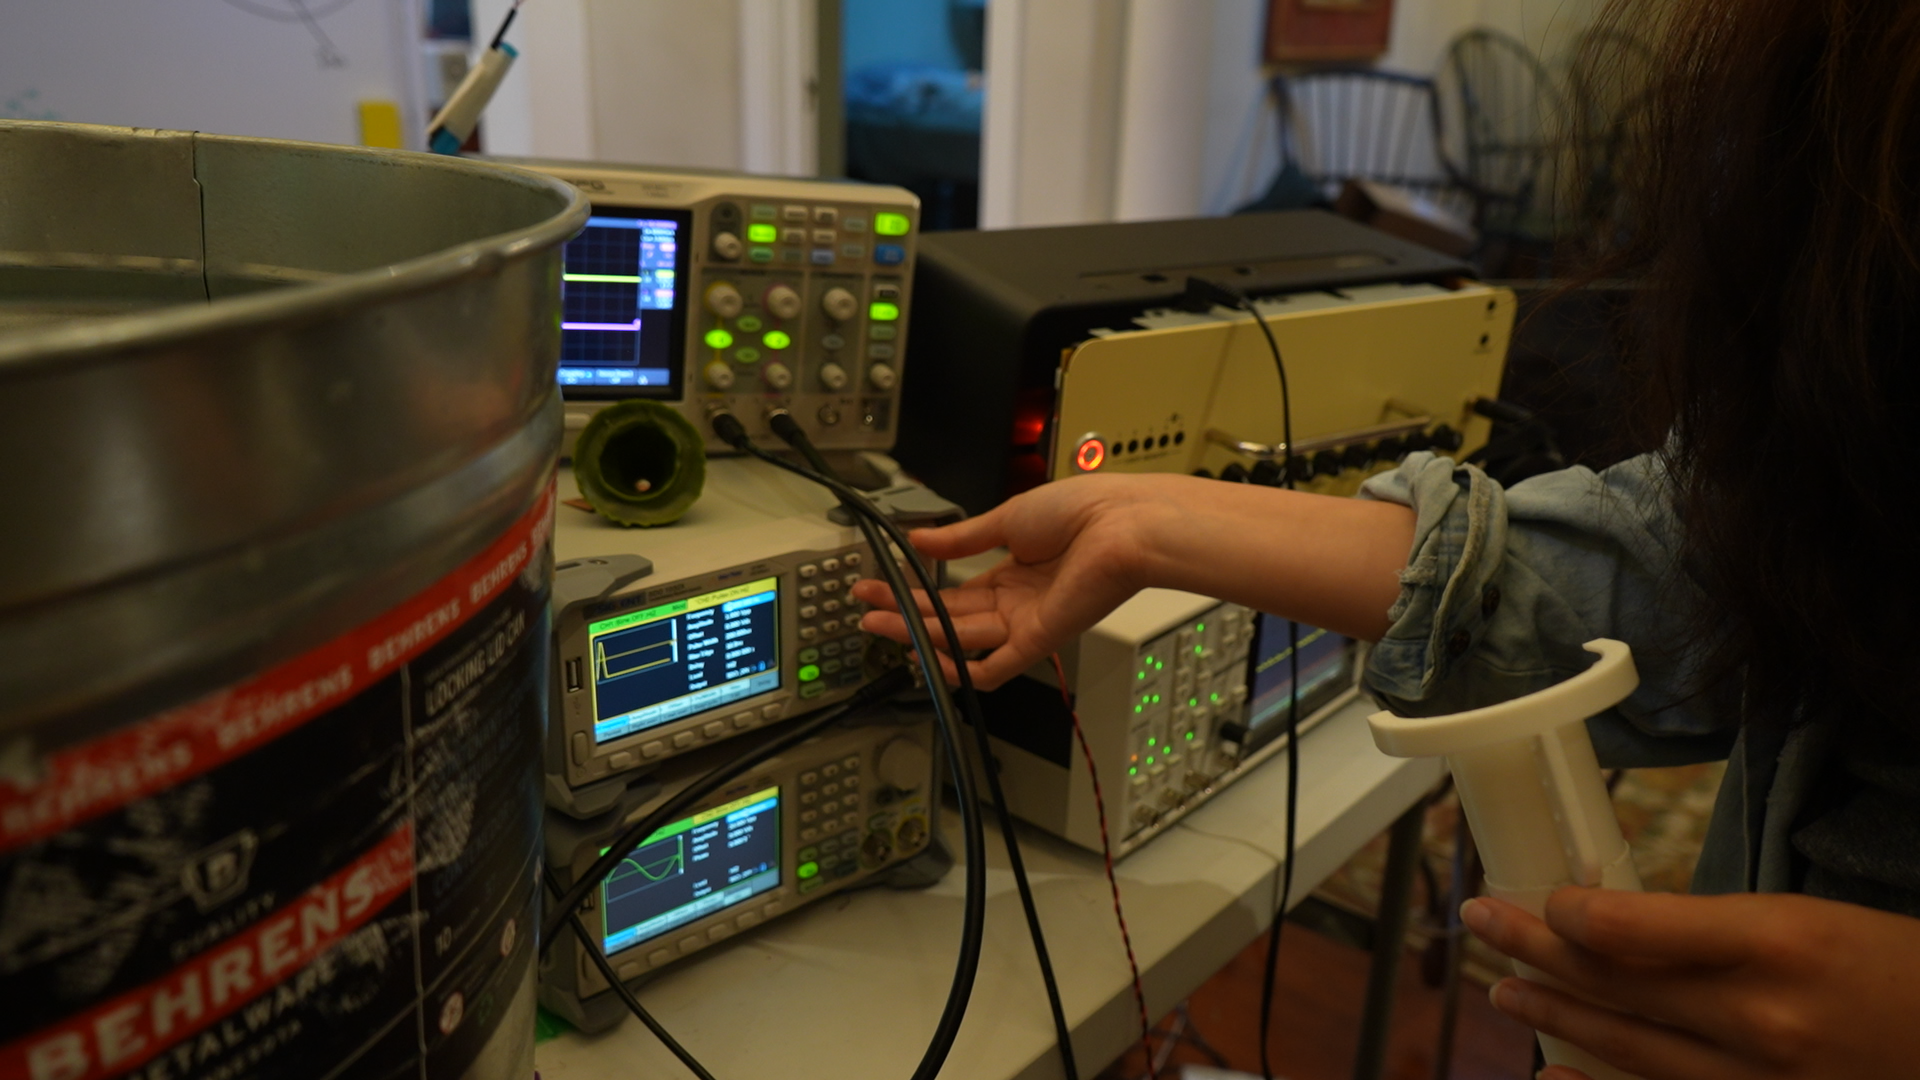
\includegraphics[width=\linewidth,height=24mm,keepaspectratio]{assets/history/brainhack-ae-workbench.png}
      \par\smallskip
      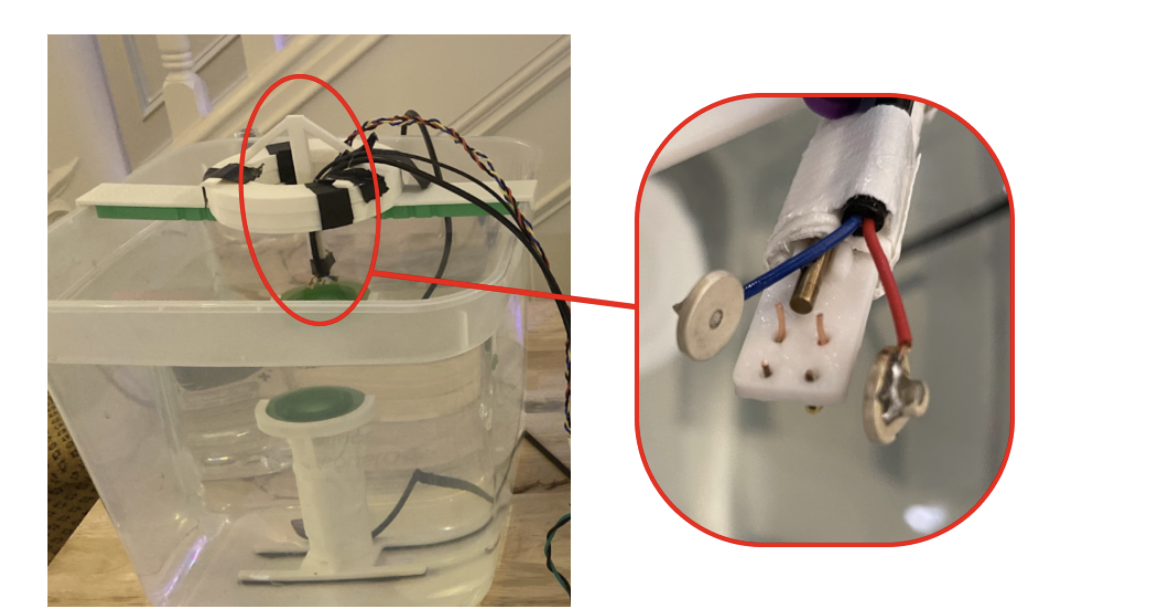
\includegraphics[width=\linewidth,height=23mm,keepaspectratio]{assets/history/brainhack-ae-probe.png}
      \par\smallskip{\scriptsize Brainhack: workbench and tank probe\par}
  \end{columns}
  {\tiny\color{NTXMuted}Sources: \href{https://reporter.mcgill.ca/meet-milo-mcgills-brain-powered-wheelchair/}{McGill Reporter}; \href{https://brainhack.vercel.app/ae}{Brainhack project}; \href{https://www.linkedin.com/posts/marley-xiong_on-thursday-we-shared-the-most-detailed-scan-activity-7476685168531988480-xSam}{Marley's Aleph announcement}\par}
  \note{[81:15--83:15] Credit the teams, not only the later founders. The Brainhack AE page names Ethan Childerhose, Kevin Chung, Andy Kong, Brian Machado, and Marley Xiong. It describes a tank experiment, not a demonstrated human neural interface. Morgan supplies the broader Brainhack-to-Aleph narrative; public sources verify these milestones and overlapping participants, not a formal spinout or a causal claim that NTX created Aleph. Aleph's brain-interface aspirations are not demonstrated telepathy. Invite Morgan's firsthand account of how relationships and shared work continued.}
\end{frame}
